\chapter{La méthode de la liaison étroite}
Jusqu'ici, on considérait que le "gaz électrons" était faiblement perturbé 
par le potentiel périodique. Un autre choix est de considérer que le solide 
est un ensemble d'atomes neutres interagissant faiblement.\\
\textsc{Exemple.} Soit un groupe d'atomes de sodium disposés en réseau 
cubique centrée avec une maille de l'ordre du cm : tous les électrons sont 
localisés. Si on les rapproche suffisamment les atomes, les $e^-$ vont ressentir 
la présence de leurs voisins et l'on obtiendra des niveaux $1s,2s,2p$ et $3s$ 
du sodium.\\

On va alors avoir des recouvrement\footnote{Lorsque deux atomes d'hydrogène se 
rapprochent, ils vont interagir. Leurs orbitales $s$ (de symétrie sphérique) vont 
se recouvrir. La région où se produit le recouvrement correspond à une augmentation 
de la densité de probabilité de trouver les électrons dans cette région de l'espace.}. 
Le recouvrement de l'état $1s$ est négligeable\footnote{??} : ces niveaux sont donc 
presque inaltérés. Pour les états $2s$ et $2p$ le recouvrement est très faible. Par 
contre, pour $3s$ (les niveaux des électrons de valence), le recouvrement est 
substantiel.\\
	\begin{wrapfigure}[14]{r}{6.5cm}
	\vspace{-0.5cm}
	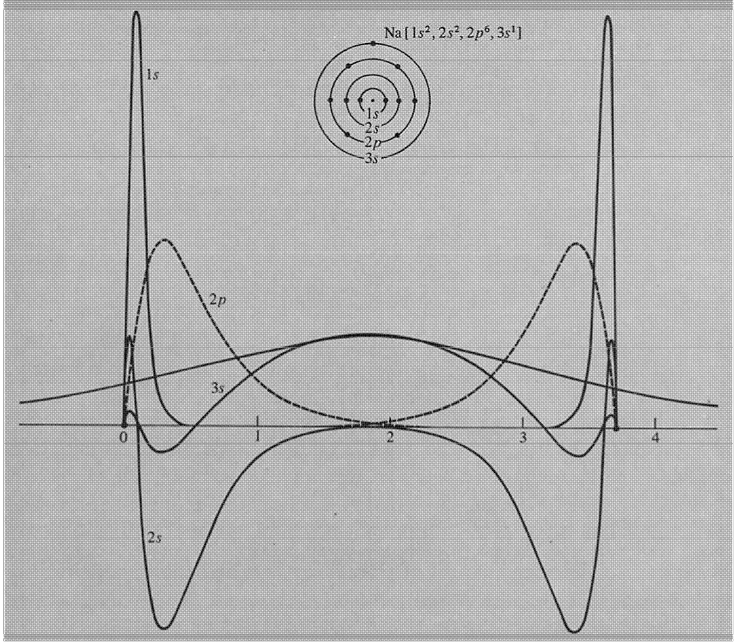
\includegraphics[scale=0.25]{ch6/image1.png}
	\captionof{figure}{ }
	\end{wrapfigure}		
Lorsque ce recouvrement est faible mais non nul, il n'est pas utile de parler de 
physique du solide mais d'utiliser l'approximation de la liaison étroite (ou 
forte). Elle traite le cas ou
\begin{enumerate}
\item Recouvrement assez important tel qu'il est nécessaire d'utiliser des correction 
par rapport au cas des atomes isolés
\item Recouvrement assez faible tel pour ne pas tout rendre absurde
\end{enumerate}
Cette approximation est utile pour décrire les bandes d'énergies des niveaux $d$ 
partiellement remplis.\\
Autrement dit, cette approximation est une différence entre un potentiel physique du 
solide et un potentiel du solide faible : les fonctions d'ondes vont ressembler à des 
états atomiques.


\section{Formulation générale}
Hypothèse : en chaque point du réseau, on peut approcher le  hamiltonien périodique 
par l'hamiltonien $H_{at}$ d'un atome isolé en ce point. Ces états liés sont bien 
localisés
\begin{equation}
H_{at}\psi_n = E_n\psi_n
\end{equation}
avec $|\psi(\vec{r})|^2$ très petit dès que $r$ dépasse l'ordre de la constante du 
réseau (\textit{range}).
L'hamiltonien $H$ du cristal s'écrit
\begin{equation}
H = H_{at} + \Delta U(\vec{r})
\end{equation}
où $\Delta U(\vec{r})$ contient les corrections pour reproduire la périodicité du 
cristal.

\danger Ici,c 'est bien parce que nous avons un atome par maille que l'on peut 
construire autour de chaque maille un état localisé (état atomique).\\

Il est donc autoriser de sommer cette fonction localisée en tenant compte un 
déphasage : ceci permettra de satisfaire la condition de Bloch. 
\begin{equation}
\psi_{nk}(\vec{r}) = \sum_{\vec{R}} e^{i\vec{k}\vec{R}}\psi_n(\vec{r}-\vec{R})
\end{equation}
où $\vec{k}$ est un des $N$ vecteurs de la première zone de Brillouin autorisé 
par les CL de BVK. On vérifie que cette fonction "somme" des états localisé 
possède les propriétés d'une fonction de  Bloch
\begin{equation}
\begin{array}{ll}
\psi_{n\vec{k}}(\vec{r}+\vec{R}) &= \sum_{R'} e^{ikR'}\psi_n(r+R-R') = \sum_{R''} 
e^{ikR}.e^{ikR''}\psi_n(r-R'')\\
&= e^{ikR}\psi_{nk}(r)
\end{array}
\end{equation}
Cependant, les bandes d'énergies ont peut de structure : $\varepsilon_n(\vec{k})$ 
est simplement l'énergie $E_n$ d'un niveau atomique, indépendant de $\vec{k}$. Pour 
y remédier, on dit que $\psi_n(\vec{r})$ est petit mais non nul quand $\Delta 
U(\vec{r})$ devient appréciable. On cherche alors une solution de la forme
\begin{equation}
\psi(\vec{r}) = \sum_{\vec{R}} e^{i\vec{k}\vec{R}}\phi(\vec{r}-\vec{R})
\end{equation}
où $\phi$ n'est pas forcément un état stationnaire exact et est à déterminer par
calcul. Si $\Delta U(\vec{r}).\psi_n(\vec{r})$ n'est pas nul mais très petit, 
$\phi(\vec{r})$ est devrait être proche de $\phi(\vec{r})$. On va supposer que 
c'est le cas pour développer $\phi(\vec{r})$ sur un petit nombre de fonctions 
d'ondes atomiques localisés :
\begin{equation}
\phi(\vec{r}) = \sum_n b_n\psi_n(\vec{r})
\end{equation}
On essaye ici de construire une sorte de "fonction d'essai" qui seront des 
fonctions de Bloch à l'aide des états atomiques (avec des paramètres 
ajustables via $b_n$).\\
\danger Les  $\psi_n$ sont des états atomiques, on ne met dans cette combili 
que ce que l'on semble être pertinent sans quoi on perdrait le sens physique : 
on va limiter $\psi_n$ aux orbitales pertinentes.\\

Reprenons notre équations de Schrödinger
\begin{equation}
H\psi(\vec{r}) = (H_{at} + \Delta U(\vec{r}))\psi(\vec{r}) = \varepsilon(\vec{k})
\psi(\vec{r})
\end{equation}
et multiplions la par une fonction d'onde atomique (en guise de "fonction d'essai") 
$\psi_m^*$ que l'on intègre sur $\vec{r}$, on doit utiliser
\begin{equation}
\int \psi_m^* H_{at}\psi(\vec{r})d\vec{r} = \int(H_{at}\psi_m)^*\psi d\vec{r} = 
E_m\int \psi_m^*(\vec{r})\psi(\vec{r})d\vec{r}
\end{equation}
pour trouver
\begin{equation}
(\varepsilon(\vec{k})-E_m)\int \psi_m^*(\vec{r})\psi(\vec{r})d\vec{r} = \int 
\psi_m^*(\vec{r})\Delta U(\vec{r})\psi(\vec{r})d\vec{r}
\end{equation}
Il faut maintenant développer $\psi(\vec{r})$ en $\phi(\vec{r})+\sum_{R'\neq 0} 
e^{ikR'}\phi(r-R')$ et utiliser $\int \psi_m^*(\vec{r})\phi(\vec{r}) = bm$ 
pour obtenir (\textit{"pas difficile, mais pas drôle non plus"}) :
\begin{equation}
\text{Équation 10.12 du A\&M, version française}
\label{eq:EqAM}
\end{equation}
Beaucoup de termes de cette expressions vont passer au bac :
\begin{itemize}
\item[$\bullet$] Le premier terme du membre de droite petit car intégrale de 
recouvrement (par  hypothèse petite)
\item[$\bullet$] Le second terme est petit car $\psi_m$ est petit quand $\Delta U$ 
est appréciable
\item[$\bullet$] Le troisième terme est petit car intégrale de recouvrement
\end{itemize}
$\Longrightarrow$ le membre de droite est petit et donc $(\epsilon(\vec{k}-E_m))b_m$ 
est petit : soit $\varepsilon(\vec{k})\approx E_m$, soit $b_m\approx 0$.
On en déduit que $\varepsilon(\vec{k}) $ est proche d'un niveau atomique, imaginons 
$E_0$ et tous les $b_m$ sont petits sauf celui associé à ce niveau :
\begin{equation}
\varepsilon(\vec{k})\approx E_0\qquad\text{et}\qquad b_m\approx0\qquad\text{sauf si}
\qquad E_m\approx E_0
\end{equation}
Connaissant cette relation aux énergies, on peut essayer d'estimer le membre de droite 
de \autoref{eq:EqAM}. Plusieurs cas sont possibles
\begin{enumerate}
\item $E_0$ est non dégénéré (état $s$) : l'équation \autoref{eq:EqAM} se réduit à une 
expression explicite de l'énergie de la bande de ce niveau (bande-s)
\item $E_0$ tripliement dégénéré (niveau $p$) : trois équations homogènes dont les 
varleurs propres donneront les $\varepsilon$ pour les trois bandes-p.
\item Pour avoir une bande-d, résoudre un problème $5\times5,\dots$
\end{enumerate}
\danger Relire page 132 !


\section{Application à une bande $s$ résultat d'un niveau atomique $s$ unique}
Supposons $b_m=0$ sauf pour un niveau atomique $s$. On vient de voir que l'on 
obtenait directement l'expression de la bande-s 
\begin{equation}
\varepsilon(\vec{k}) = +E_s-\dfrac{\beta+\sum \gamma(\vec{R})e^{i\vec{k}\vec{R}}}{
1+\sum \alpha(\vec{R})e^{i\vec{k}\vec{R}}}
\end{equation}
où $E_s$ est l'énergie du niveau atomique $s$. Comme les $\alpha(\vec{r})$ ne 
donnent que de faibles corrections, on va les négliger.\footnote{Justif?} De plus, 
on suppose que le recouvrement ne se fait qu'entre les plus proches voisins : 
\begin{equation}
\varepsilon(\vec{k}) = E_s-\beta -\sum_{\text{proches \ voisins}} \gamma(\vec{R})
\cos\vec{k}.\vec{R}
\end{equation}
où $\vec{R}$ du réseau de Bravais connecte l'origine à ses plus proches voisins. 
On compte 12 plus proches voisins :
\begin{equation}
\vec{R} = \dfrac{a}{2}(\pm1,\pm1,0),\quad \frac{a}{2}(\pm1,0,\pm1),\quad \frac{a}{2}
(0,\pm1,\pm1).
\end{equation}
Si $k=(k_x,k_y,k_z)$, les valeurs de $\vec{k}.\vec{R}$ correspondantes sont
\begin{equation}
\vec{k}.\vec{R} = \frac{a}{2}(\pm k_i,\pm k_j)\qquad i,j = x,y;y,z;z,x
\end{equation}
Or $\Delta U(x,y,z)$ est inchangé par permutation d'arguments/signes. Comme 
$\psi_s(\vec{r})$ ne dépend que de $r$, $\gamma(\vec{R})$ est la même constante 
pour les 12 vecteurs $\vec{R}$. On a donc
\begin{equation}
E(\vec{k}) = E_s-\beta-4\gamma\left(\cos\frac{k_xa}{2}\cos\frac{k_ya}{2}+
\cos\frac{k_ya}{2}\cos\frac{k_za}{2}+\cos\frac{k_za}{2}\cos\frac{k_xa}{2}\right)
\end{equation}



















